\documentclass[11pt, a4paper]{article}
\usepackage[margin = 2cm]{geometry}
\setlength{\parskip}{0cm}
\setlength{\parindent}{1cm}
\usepackage[compact]{titlesec}
\titlespacing{\section}{0pt}{1ex}{1ex}
\titlespacing{\subsection}{0pt}{1ex}{0ex}
\titlespacing{\subsubsection}{0pt}{0.5ex}{0ex}
\usepackage[utf8]{inputenc}
\usepackage{fontspec}
\setmainfont{Arial}
\usepackage{graphicx}
\usepackage{lineno}
\usepackage{float}
\usepackage[font=small,labelfont=bf]{caption}
\usepackage{setspace}
\onehalfspacing

\begin{document}
    \begin{titlepage}
	\center
	
\includegraphics[width=0.5\textwidth]{imperial.png}\par\vspace{1cm}
	\vspace{1cm}
	MSc COMPUTATIONAL METHODS IN ECOLOGY AND EVOLUTION
	\vspace{1cm}
	
	\rule{\linewidth}{0.5mm}
	{\Large\bfseries Project Proposal: Joint Estimation of Population Size and Migration Rate for Mosquito Population Control\par}
	\rule{\linewidth}{0.5mm}
	
	\vspace{1cm}


    \begin{minipage}{0.4\textwidth}
    \begin{flushleft} \large
    \emph{Author:}\\
    Sam TURNER\\
    \emph{CID:}\\
    01804283
    \end{flushleft}
    \end{minipage}
    \begin{minipage}{0.4\textwidth}
    \begin{flushright} \large
    \emph{Primary Supervisor:} \\
    Austin BURT \\    Department of Life Sciences\\
    a.burt@imperial.ac.uk
    \end{flushright}
    \end{minipage}\\[1cm]
    {\large \today}\\[0.5cm] 
    \vfill
    \newpage
    \end{titlepage}
    
\begin{linenumbers}
\section*{Key Words}
\noindent Population genetics; Joint parameter estimation; Genome simulation; Mosquito population structure; Migration rates; Sampling strategies

\section*{Project Idea and Proposed Questions}
\noindent Female Anopheles mosquitos transmit malaria, causing around 400,000 deaths globally each year, 70\% of which are children under 5 \cite{WHO_report}. Whilst population control of Anopheline mosquitos has been effective in reducing this burden \cite{historical_review}, widespread elimination using current strategies (primarily bednetting and IRS) is unlikely. The desired scaling up of this strategy, requiring an increase in funding from \$2.7bn to \$9bn per year, is still predicted leave malaria in 62 countries by 2030 \cite{griffin}. As such, there is renewed interest in genetic methods for population control: a promising approach is the use of homing endonuclease genes (HEGs), which use gene drive to allow a lethal or sterilising genetic construct to spread through a population \cite{burt}.

The evaluation of genetic control strategies is requires an understanding of the population genetics of the target species. In this project, we aim to develop a method for jointly estimating effective population size and migration rates. These parameters are of central interest to HEG work, allowing modelling of construct spread and evolution of host resistance.

Methods for estimating recent population size of closed populations exist, often based on allele frequency fluctuations \cite{Waples1989}, or linkage disequilibrium \cite{hill_1981}. However, mosquitos are known to exist in structured population \cite{ag1000nature}, posing a challenge for parameter inference: migration has been shown bias population size estimates from both allelic fluctuation \cite{wang} and linkage disequilibrium \cite{waples2011} based methods.

We aim to study the effect of population structure on the outcome on a number of population size estimators. Further, differences in the effect of migration on these estimators may allow us to construct a method for joint estimation of population size and migration rate. By analysing the properties of the joint estimator, we aim to determine how sampling strategy affects the confidence of parameter estimates, informing decisions on the sampling strategy used to collect mosquito genomes.

\section*{Proposed Methods}	
\noindent We will examine the properties of preexisting population size estimators, both analytically and with simulation, which may lead to an analytically derived joint estimator. Further, the simulated genomes can directly be used for joint estimation. The properties of the joint estimator can then be studied both analytically and with simulation

\paragraph{Genome Simulation}
Simulation of genomes using the coalescent has become an important part of population genetics \cite{msprime}, and will be used to test the behaviour of estimators. Here, we will produce coalescent trees using msprime \cite{msprimearticle}, which represent samples from an idealised population under a range of demographic scenarios: this includes varying population sizes, migration rates, and migration patterns.

\paragraph{Examining Estimator Behaviour}
We will examine the behaviour of estimators both analytically and via simulation. In the analytic approach, the properties of estimators are expressed as a function of the parameters of interest. The validity of the derived relationships can then be tested using genomes simulated under known demographic scenarios. However, quantities such as the variance or distribution of estimators may be difficult to determine analytically, so may be approximated by applying the estimator to simulated genomes. In particular, the response of bias and variance to sampling strategy will be of interest.

\paragraph{Joint Estimation}
The difference between preexisting estimators may be a useful statistic for estimating migration rate and population size. If so, we will construct a joint estimator using either analytical (maximum likelihood, method of moments \cite{wang}) or algorithmic (Approxmiate Bayesian Computation \cite{abc}) approaches. Similarly, the ratio of a single estimator taken in different demes may also hold information that allows a joint estimator to be constructed.

\section*{Outputs and outcomes}
\noindent Estimates of population size and migration rate are critical for HEG modelling. This project aims both to produce an estimator, and to determine how sequencing resources can best be allocated to provide precise parameter estimates. In particular, the group is involved with the Ag1000 project, which has sequenced 1142 \textit{A. gambiae} genomes to date \cite{ag1000preprint}. These have uncovered structured local populations with gene flow and varying effective size, which must be quantified for genetic control mechanisms to be evaluated \cite{ag1000preprint}. To this end, Ag1000 will be sequencing many more genomes, the allocation and analysis of which can be informed by this work. 

\section*{Timeline and Feasibility}
\noindent The simulation and mathematical techniques which we propose to use are well established, and have been used in similar estimation work before, including in this group \cite{Hui}. It is highly likely that a set of estimators can be found that jointly give information on population size and migration rate, although it is possible that analytical estimator construction will be harder. However, numerical alternatives using simulation are available, so it is very feasible that a sound estimator is produced by the end of the project. 
Also, the current requirement for remote working will not be problematic as the work is computational, with communication possible over email, telephone, or video call. 
        \begin{figure}[H]
        \centering
        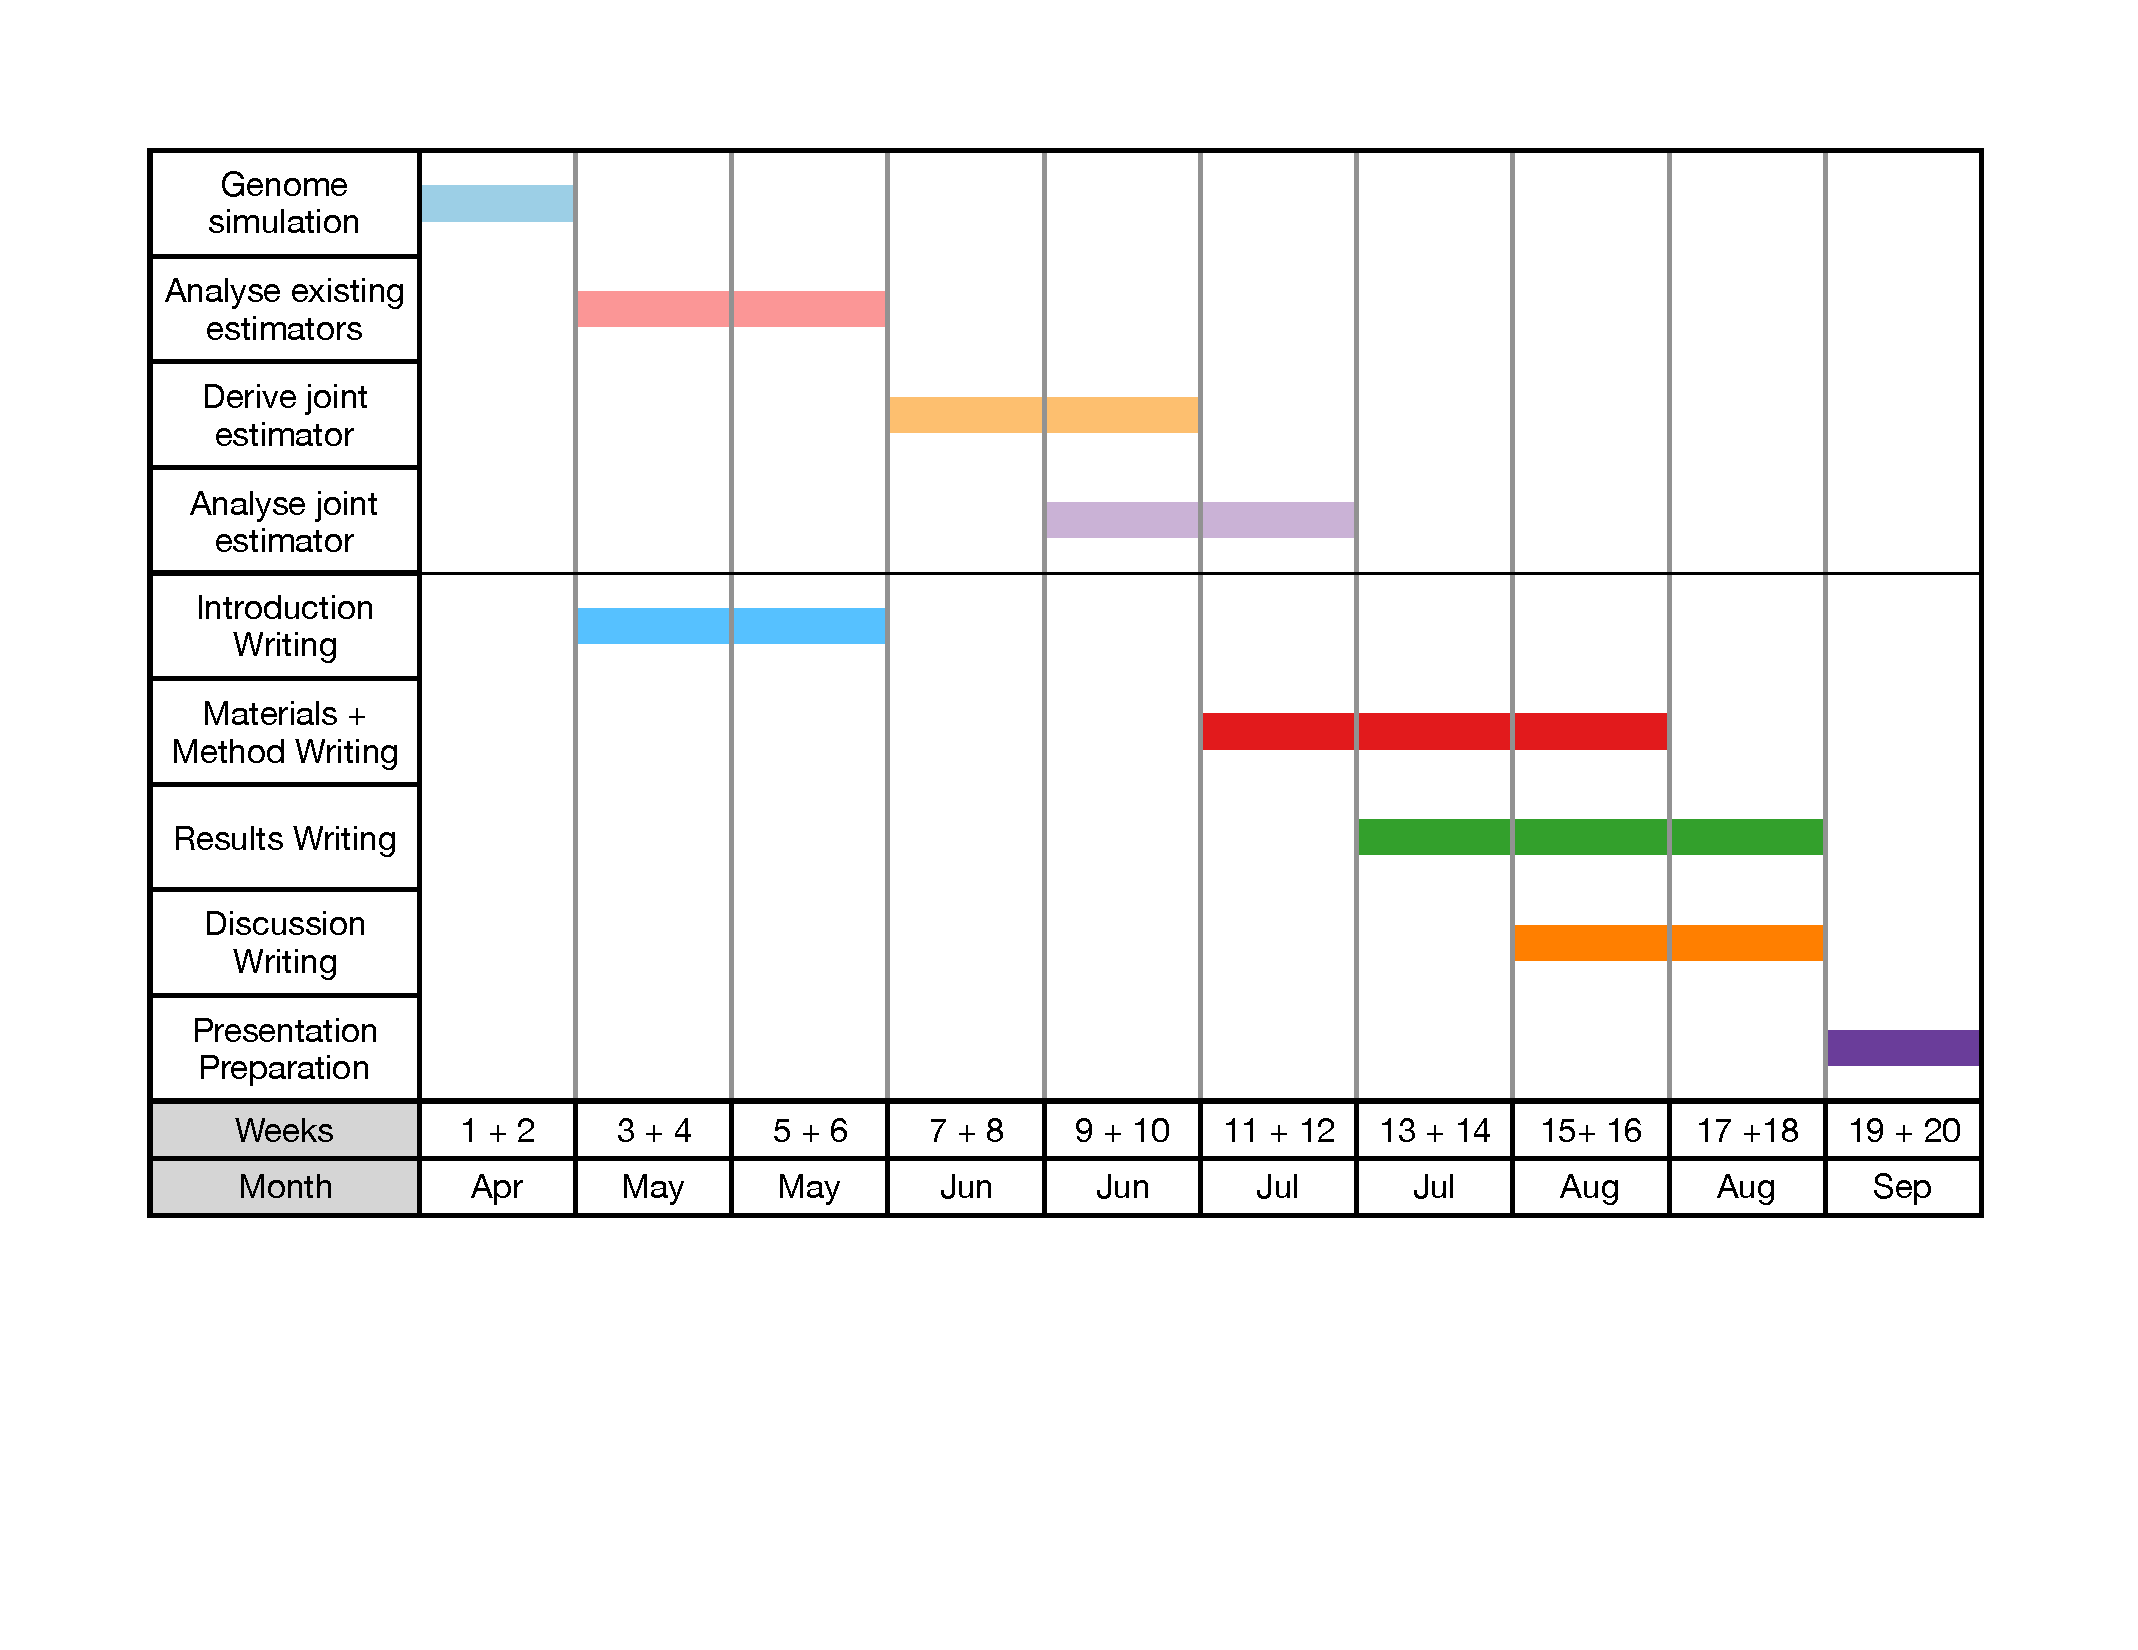
\includegraphics[width=4in]{Gantt.pdf}
        \caption{ Gantt chart showing timeline for project completion.}
        \label{fig:gannt}
        \end{figure}
\section*{Budget}
\paragraph{High performance computing time: £500}
Extensive use of Imperial’s HPC services will be required as coalescent simulation is computationally expensive, with many simulations required to densely cover the parameter space for Approximate Bayesian Computation. 
\end{linenumbers}

\bibliographystyle{apalike}
\bibliography{proposal}

\newpage
\section*{Declaration}
\vspace{1cm}
{"I have seen and approved the proposal and the budget"}\\
\vspace{1cm}




\begin{tabular}{@{}p{.5in}p{4in}@{}}
Approved: & \hrulefill \\
& Austin BURT \\
& \today \\
\end{tabular}




\end{document}
